\documentclass[a4paper,11pt,fleqn]{scrartcl}%fleqn pour aligner les equations à gauche
\usepackage{../../Styles/Exercice}

\newcommand{\chnum}{Chapitre 13}
\newcommand{\chtitle}{Mouvement et forces}
\newcommand{\dtype}{Exercices}

\begin{document}
\maketitle

\begin{multicols}{2}
\section{Connaître la direction et le sens de $\sum \vec{F}$}

Pour les tableaux ci-dessous, relier chaque schéma de $\Delta \vec{v}$ et $\vec{v}$ à la somme des forces $\sum \vec{F}$ qui lui correspond. Plusieurs schémas peuvent accepter la même réponse.
\begin{center}
\begin{tabular}{ccm{3cm}cc}
%\hline
A &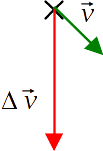
\includegraphics[scale=0.3]{Ressources/EX1_A.png} & &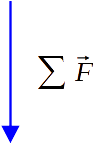
\includegraphics[scale=0.3]{Ressources/EX1_1.png}&1\\
%\hline
B &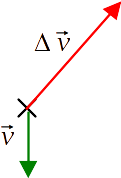
\includegraphics[scale=0.3]{Ressources/EX1_B.png} & &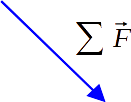
\includegraphics[scale=0.3]{Ressources/EX1_2.png}&2\\
%\hline
C &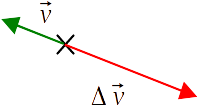
\includegraphics[scale=0.3]{Ressources/EX1_C.png} & &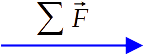
\includegraphics[scale=0.3]{Ressources/EX1_3.png}&3\\
%\hline
D &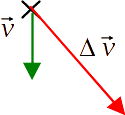
\includegraphics[scale=0.3]{Ressources/EX1_D.png} & &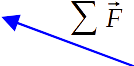
\includegraphics[scale=0.3]{Ressources/EX1_4.png}&4\\
%\hline
\end{tabular}
\end{center}

\section{Exploiter la somme des forces $\sum \vec{F}$}
Un mobile relié par un fil à un plot central fixe est lancé. Le fil reste tendu au cours du mouvement du mobile qui se déplace sans frottement sur un support horizontal. On a représenté ci-dessous les positions occupées par le mobile à intervalles de temps égaux ainsi que la comme des forces $\sum \vec{F}$ appliquées à ce mobile en quatre positions A, B, C et D.\\
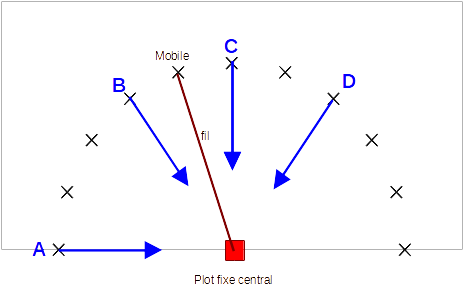
\includegraphics[scale=0.5]{Ressources/EX2.png}

\begin{picture}(0,0)
\line(5,1){5}
\end{picture}

\begin{enumerate}
\item Décrire le mouvement du mobile
\item Représenter le vecteur variation de vitesse $\Delta \vec{v}$ sans contrainte d'échelle aux positions A, B, C et D.
\end{enumerate}

\columnbreak
\section{Connaître l'influence de la masse du système}
Un système assimilé à un point M de masse $m$ glisse sur le sol. Il est soumis aux forces représentées ci-dessous à la même échelle.\\
La force $\vec{f}$ est une force de traction constante tout au long du mouvement.
\begin{enumerate}
\item Schématiser la somme $\sum{\vec{F}}$ des forces.
\item En déduire, d'après la relation approchée $\sum{\vec{F}}=m \cdot \frac{\Delta \vec{v}}{\Delta t}$, la direction et le sens du vecteur variation de vitesse $\Delta \vec{v}$ et le représenter sans contrainte d'échelle.
\item Un autre système de masse $2m$ est soumis à cette même somme des forces. Pour une même durée, comparer les vecteurs variation de vitesse de ces deux systèmes.
\end{enumerate}

\begin{center}
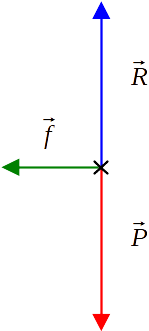
\includegraphics[width=.2\linewidth]{Ressources/EX3.png}
\end{center}

\section{Connaître l'influence de la masse (encore)}
Dans les deux situation schématisées ci-dessous, les deux systèmes, respectivement de masse $m$ et $m+m'$, sont soumis à la même somme des forces $\sum{\vec{F}}$. Les vecteurs variation de vitesse ont été représentés avec la même échelle.\\
\begin{center}
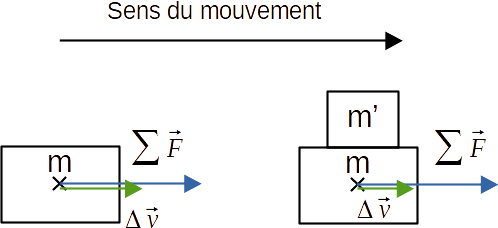
\includegraphics[width=.7\linewidth]{Ressources/EX4.png}\\
\end{center}
Justifier la différence entre les deux vecteurs variation de vitesse.

\pagebreak
\section{Thrust}
The force which moves any aircraft through the air is generated by the propulsion system of the aircraft: a fluid is ejected by the system and the ejection reaction produces a force on the system, called \textbf{thrust}.\\
\textit{Vocabulary : thrust: poussée}\\

\begin{enumerate}
\item Give the direction and sens of the speed variation vector in the accelerated rectilinear motion of the aircraft.
\item Deduce the direction and sense of the vector sum of the forces exerted on the aircraft.
\item Considering that the sum of the forces is equivalent to the only force of propulsion, in what direction is the thrust of the airplane?
\end{enumerate}

\section{Trampoline}
On s'intéresse au mouvement vertical vers le bas d'un athlète de 70 kg, après avoir atteint le  sommet de sa trajectoire, lors d'un saut sur un trampoline. Ce mouvement a une durée de 1,0 s. On considère que l'air n'a aucune action sur l'athlète.
\begin{itemize}
\item Quelle est la valeur de la vitesse de l'athlète lorsqu'il retombe  sur le trampoline?
\end{itemize}
\end{multicols}
\end{document}